\chapter{Interfaccia Utente}

L’interfaccia utente è stata progettata per essere intuitiva e facile da usare, permettendo all' utente
finale di interagire con il sistema e gestire i propri dispositivi in modo
semplice e veloce.

\section{Implementazione frontend}

Il frontend è stato sviluppato utilizzando il framework React (analizzato in dettaglio nel capitolo 5.1.3).
Esso consente la creazione di interfacce utente dinamiche e reattive, 
in grado di rispondere agli input dell'utente in tempo reale.
Il codice è stato suddiviso in componenti riutilizzabili, ognuno dei quali
racchiude una funzionalità specifica.
Mantine~\cite{mantine_website} è stato utilizzato come libreria di componenti per la creazione di interfacce utente.

\subsection{Struttura del codice}

Il progetto del frontend presenta la seguente struttura di cartelle:

\begin{itemize}
    \item \texttt{js}: contiene i file di utility e serviceWorker.
    \item \texttt{components}: contiene i componenti React riutilizzabili.
    \item \texttt{views}: contiene le pagine principali dell'applicazione.
    \item \texttt{services}: contiene i servizi per la comunicazione con il server.
    \item \texttt{rhai\_interop}: contiene un modulo stub per l'interoperabilità js con Rhai.
\end{itemize}

\section{Overview dell'interfaccia}

\subsection{Pagina di login e registrazione}

\begin{figure}[H]
    \centering
    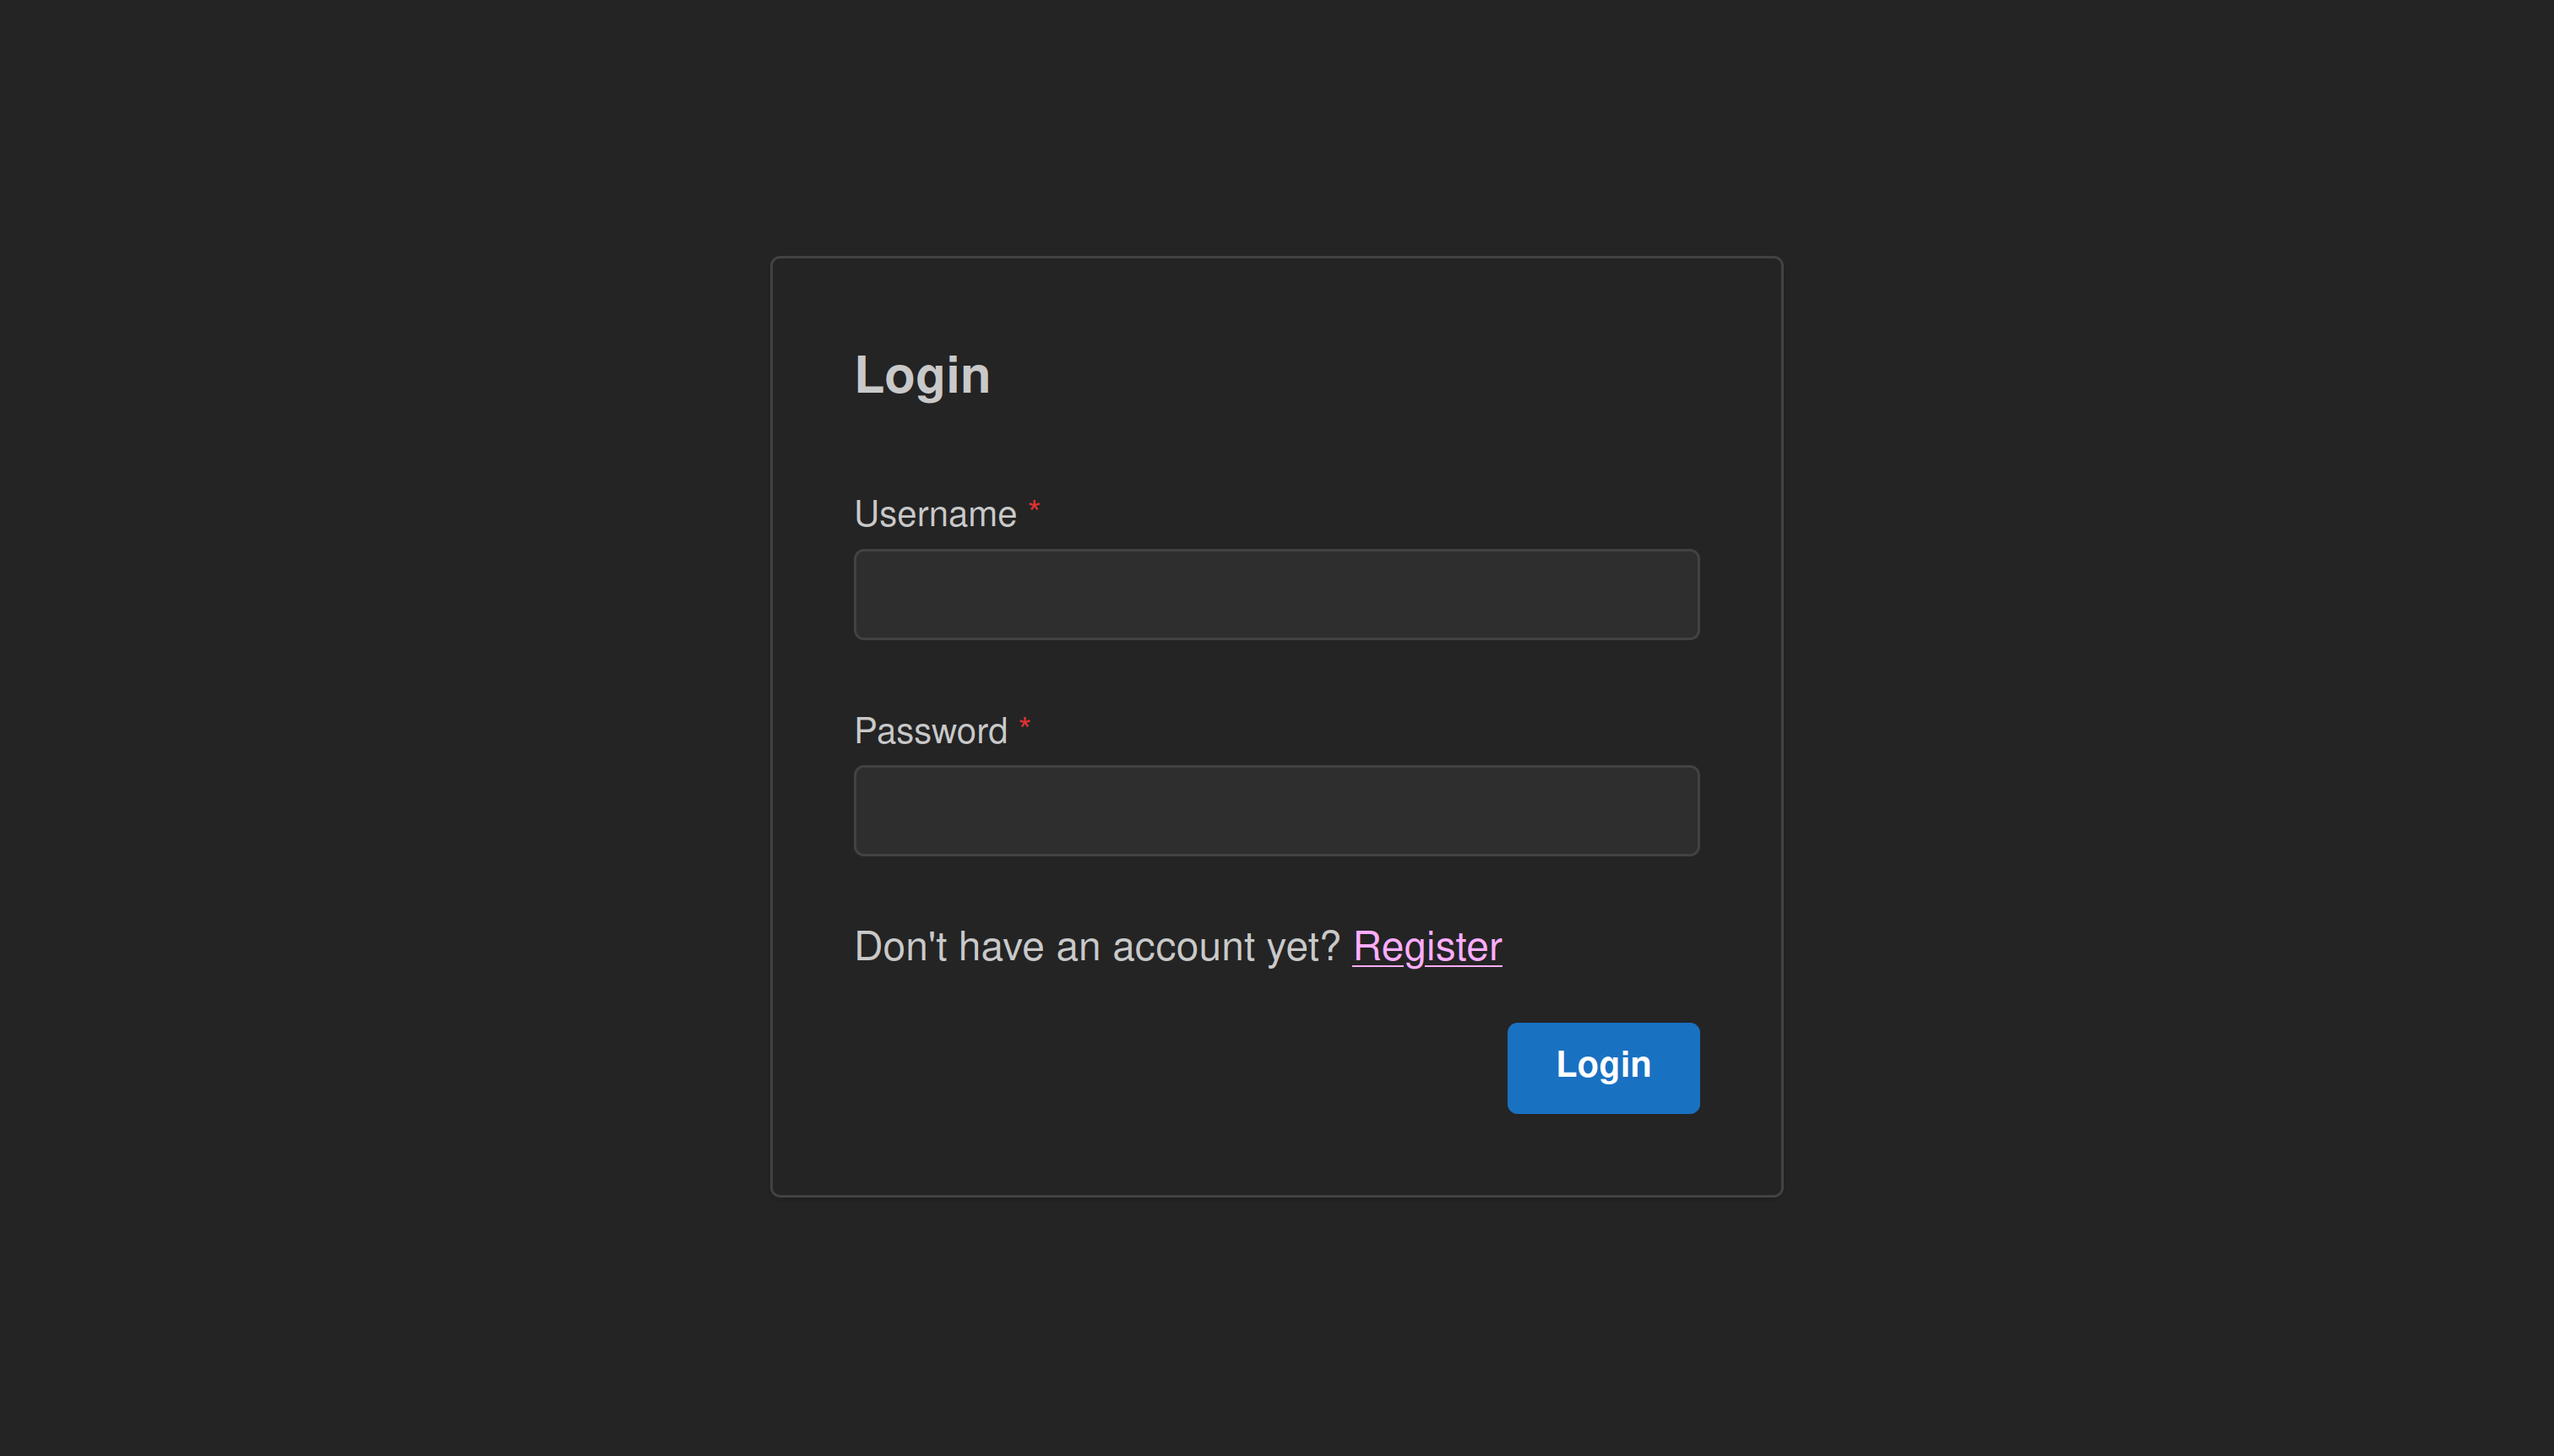
\includegraphics[width=0.8\textwidth]{images/chapter7/login.png}
    \label{fig:login}
  \end{figure}

Lo stesso componente \texttt{SignForm} è utilizzato sia per la registrazione che per il login. 
Esso presenta una semplice interfaccia con due campi di testo per l'inserimento di email e password,
e un pulsante per la conferma.

\subsection{Dashboard}

\begin{figure}[H]
    \centering
    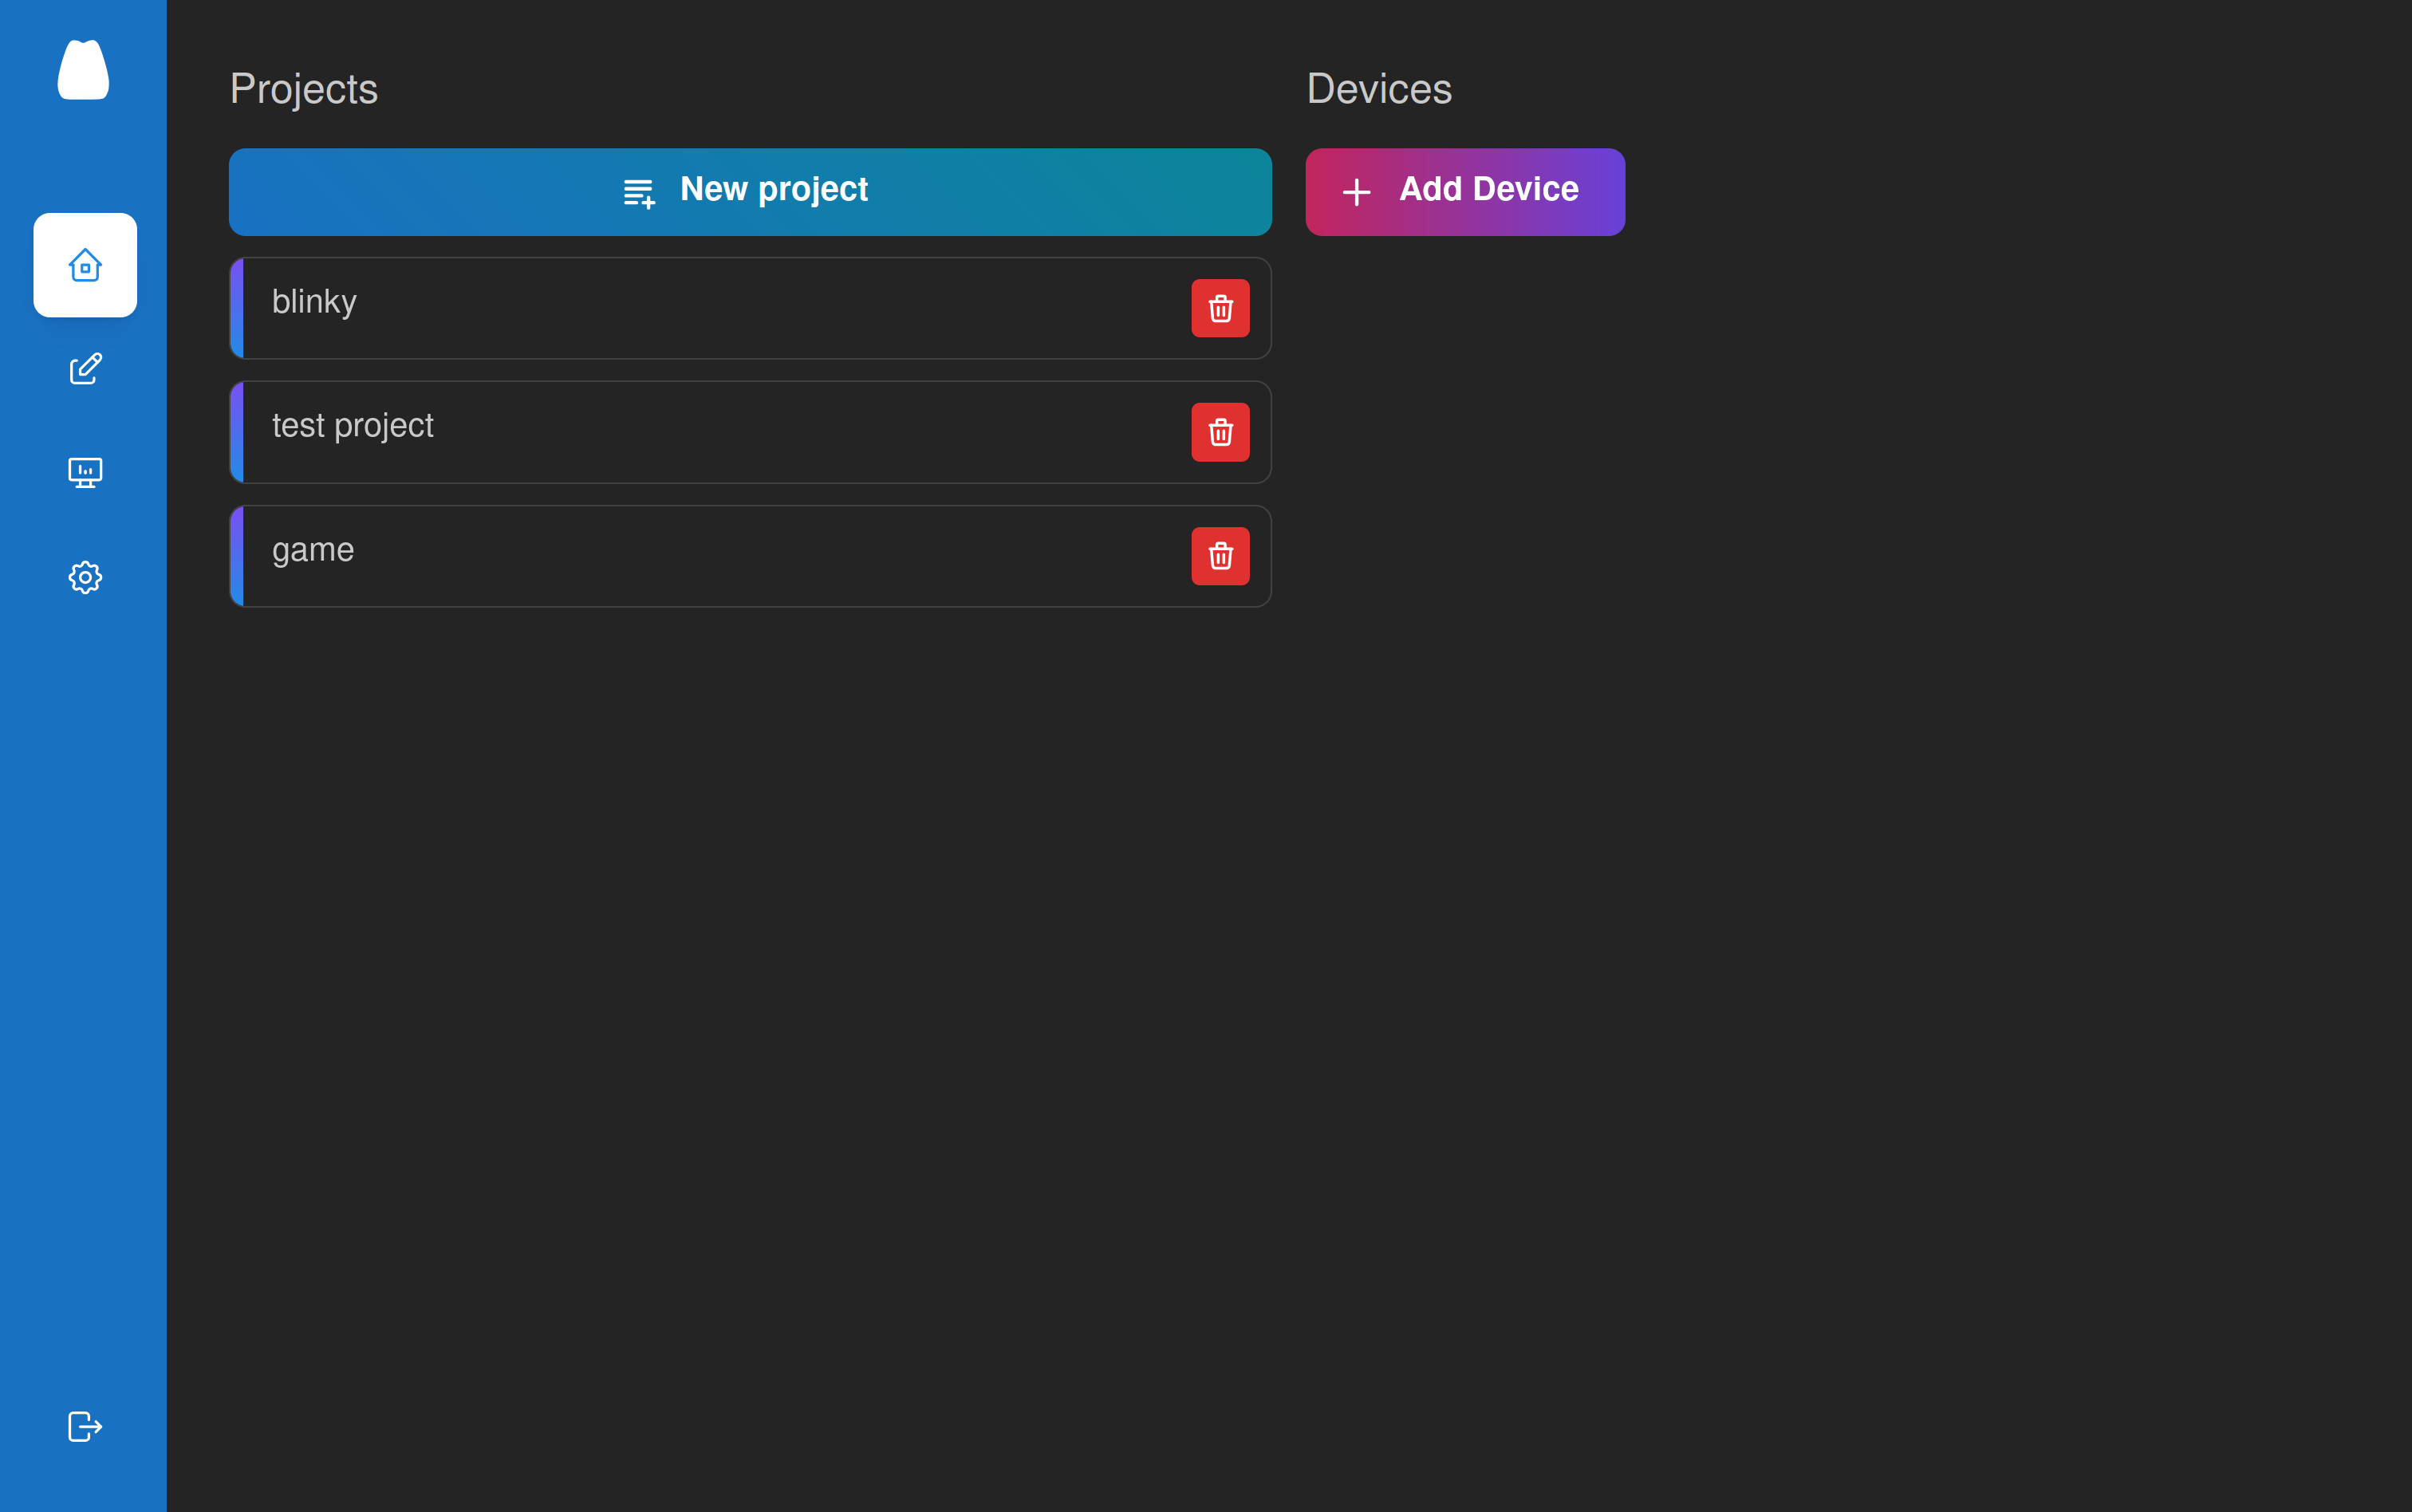
\includegraphics[width=0.8\textwidth]{images/chapter7/dashboard.png}
    \label{fig:dashboard}
  \end{figure}

La dashboard è la pagina principale dell'applicazione, viene aperta dopo che l'utente ha effettuato il login 
e contiene la lista di progetti e dispositivi associati all'utente.

\subsection{IDE e simulatore}

\begin{figure}[H]
    \centering
    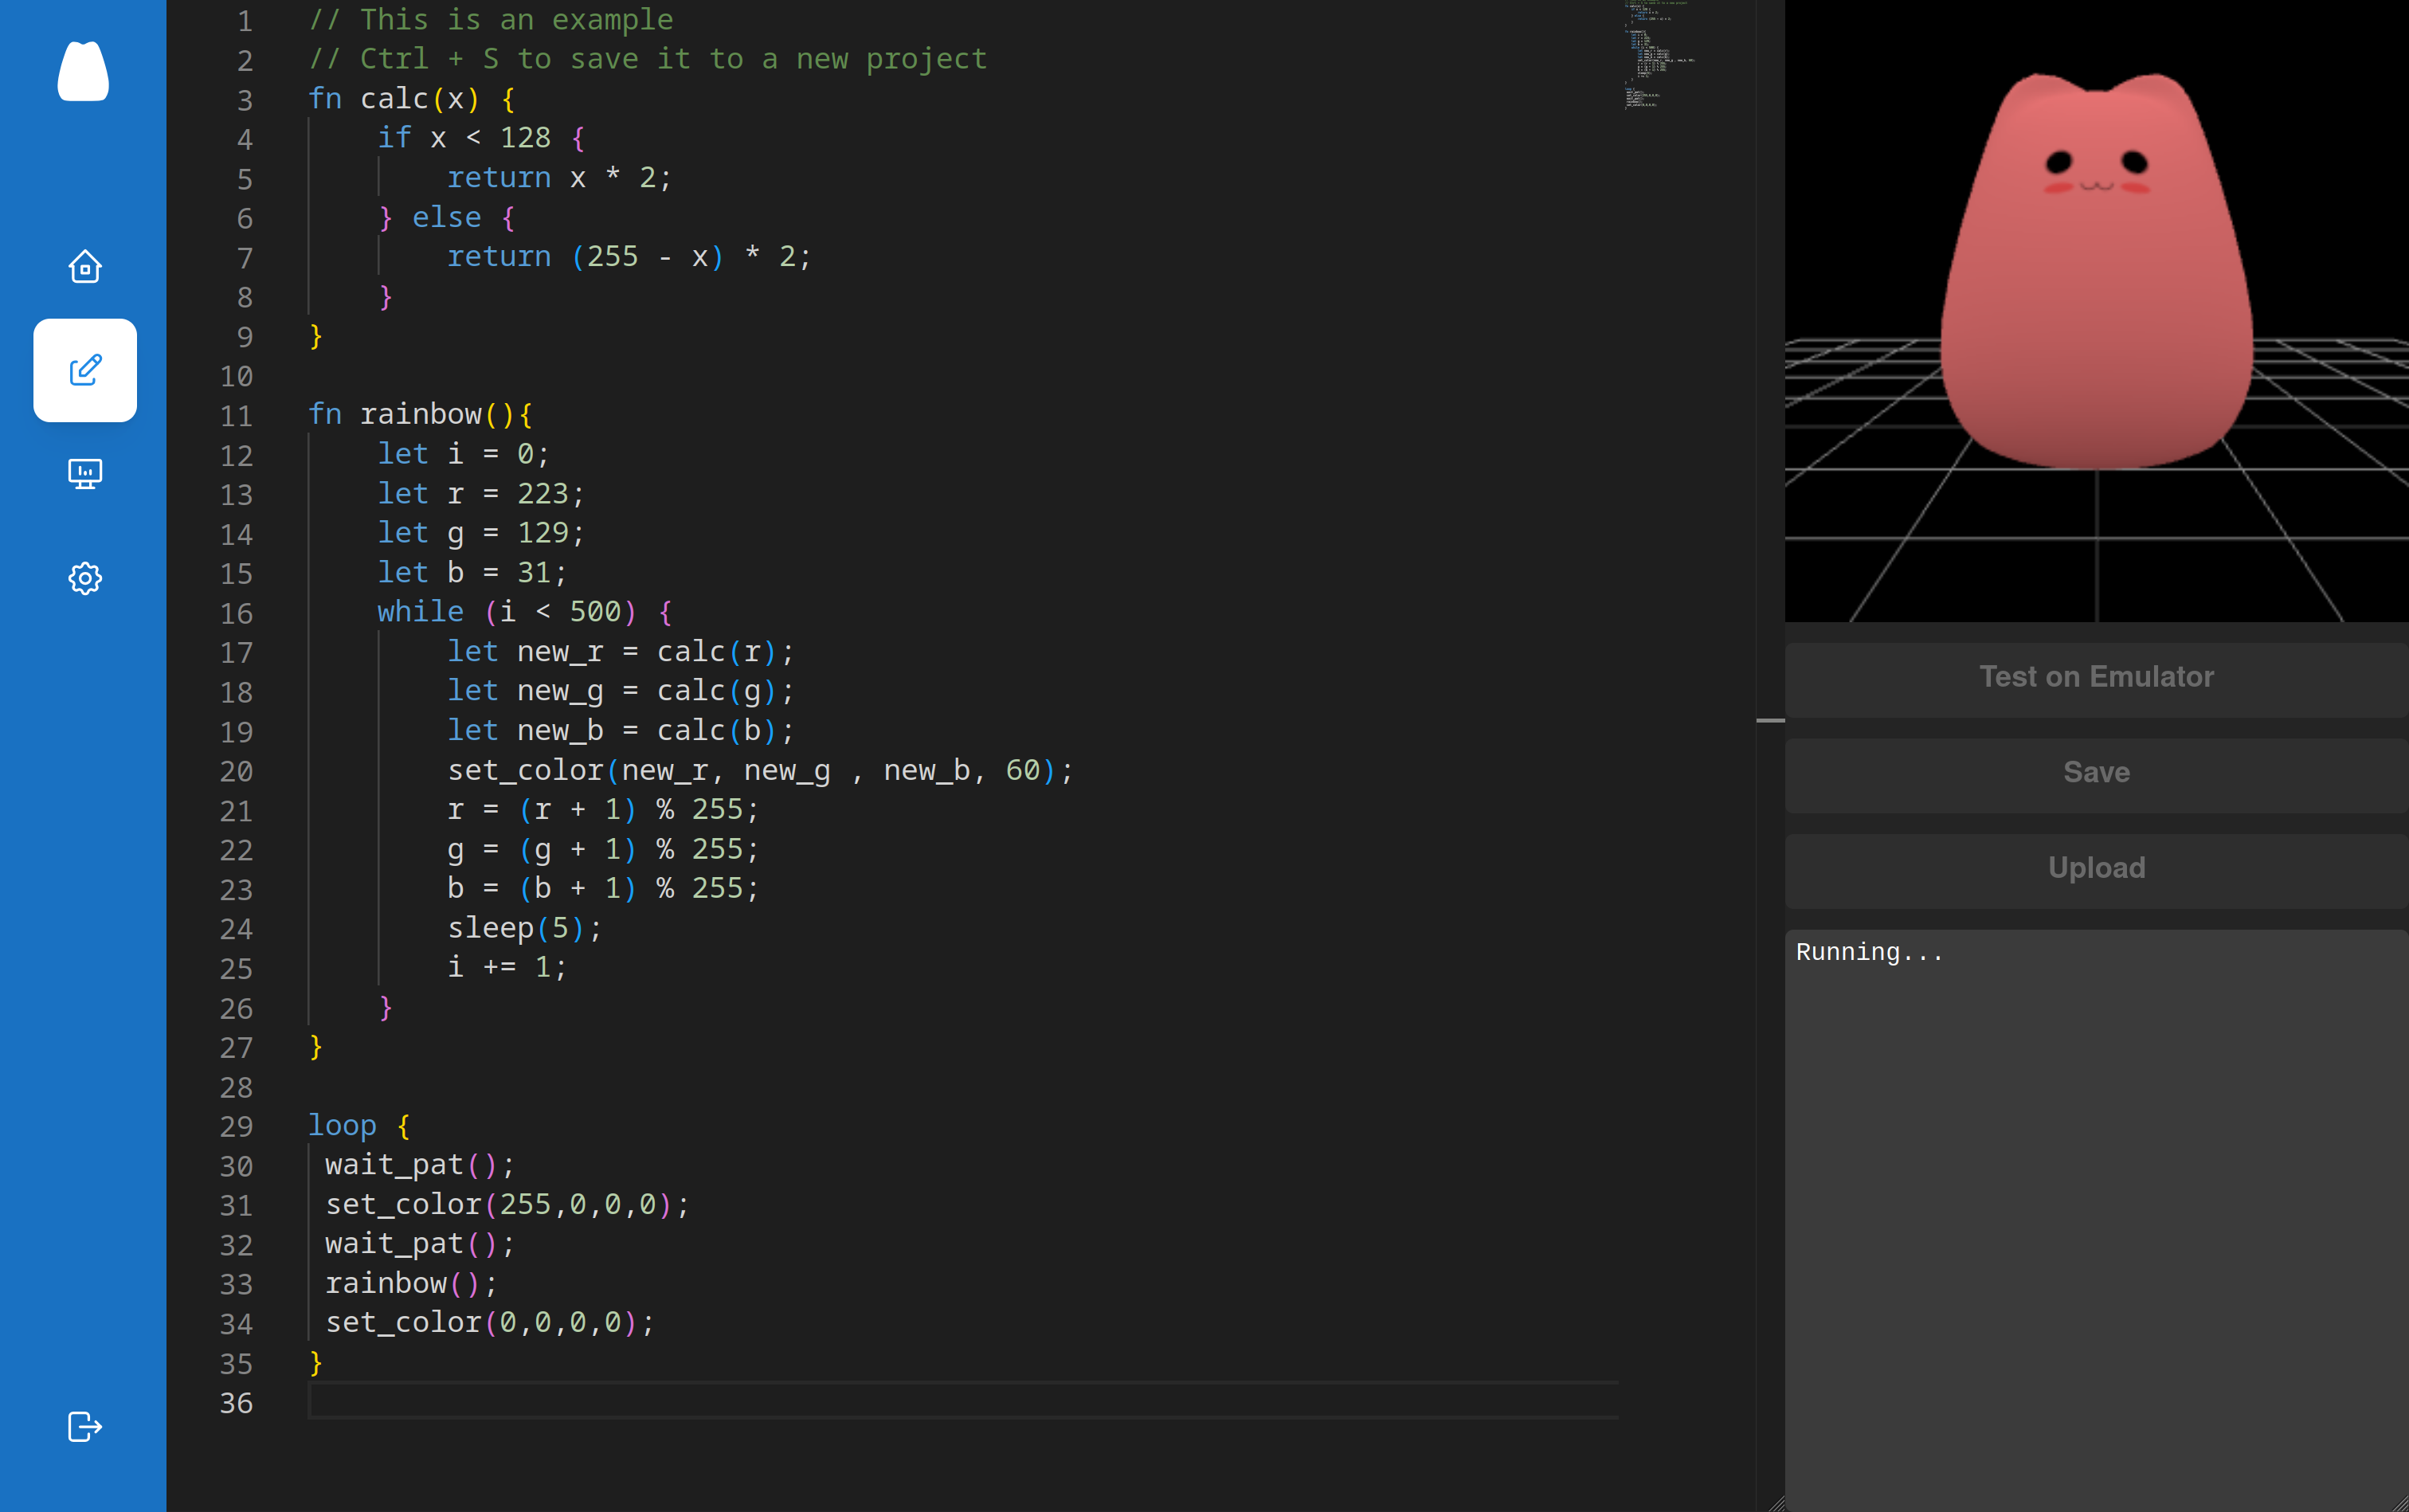
\includegraphics[width=0.8\textwidth]{images/chapter7/ide.png}
    \label{fig:ide}
  \end{figure}

L'IDE è una pagina che permette all'utente di scrivere codice Rhai, salvarlo all'interno 
di un progetto, testarlo attraverso il simulatore e caricarlo sul dispositivo target.
Il simulatore è rappresentato dal modello 3D del dispositivo che reagisce in tempo reale
alle azioni dell'utente.

L'editor di codice è stato realizzato utilizzando \texttt{monaco-editor}, l'editor di codice sorgente open-source di Visual Studio Code~\cite{monaco-editor}.
è possibile inoltre visualizzare i log e gli errori generati dall'esecuzione del codice.